\makeatletter
\def\input@path{{../styles/}{../../styles/}{../../../styles/}{../}{../../}{../../../}}
\makeatother
\documentclass{ee102_notes}
% macros.tex - Course meta information
\renewcommand{\course}{EE 102}
\renewcommand{\coursetitle}{Signal Processing and Linear Systems}
\renewcommand{\instructor}{Ayush Pandey}
\renewcommand{\semester}{Fall}
\renewcommand{\year}{2025}
\renewcommand{\shorttitle}{Week 1: Introduction to Signals}
% Use \renewcommand to avoid 'already defined' errors

% The following packages can be found on http:\\www.ctan.org
% \usepackage{graphics} % for pdf, bitmapped graphics files
%\usepackage{epsfig} % for postscript graphics files
%\usepackage{mathptmx} % assumes new font selection scheme installed
%\usepackage{times} % assumes new font selection scheme installed
\usepackage{amsmath} % assumes amsmath package installed
\usepackage{amssymb,mathtools}  % assumes amsmath package installed
\usepackage{xcolor}
\usepackage{pgfplots,subcaption}
\usepackage[hidelinks]{hyperref}
\usepackage{verbatim}
\usepackage{graphicx}
\usepackage{listings}
\usepackage{fancyhdr}
% \usepackage{geometry}
\usepackage{siunitx}
\usepackage[most]{tcolorbox}
\usepackage{enumitem}
\usepackage{environ}
% -------- listings (Python) ----------
\lstdefinestyle{py}{
  language=Python,
  basicstyle=\ttfamily\small,
  keywordstyle=\color{blue!60!black}\bfseries,
  commentstyle=\color{green!40!black},
  stringstyle=\color{orange!60!black},
  showstringspaces=false,
  columns=fullflexible,
  frame=single,
  framerule=0.3pt,
  numbers=left,
  numberstyle=\tiny,
  xleftmargin=1em,
  tabsize=2,
  breaklines=true,
}

\usepackage[american]{circuitikz}
\usepackage{tikz}
\usetikzlibrary{arrows.meta,positioning,calc,angles,quotes}
\tikzset{
  >={Latex[length=2.2mm]},
  block/.style={draw, thick, rectangle, minimum height=10mm, minimum width=24mm, align=center},
  gain/.style={block, minimum width=14mm},
  sum/.style={draw, thick, circle, inner sep=0pt, minimum size=6mm},
  conn/.style={-Latex, thick},
}
\usepackage{caption}    
\usepackage{lscape}
\usepackage{soul}
\usepackage{physics}
\usepackage{hyperref}
\hypersetup{
    colorlinks=true,
    linkcolor=blue,
    filecolor=magenta,      
    urlcolor=blue,
    pdftitle={week1_notes},
    pdfpagemode=FullScreen,
}
%\usepackage{float} 

%\usepackage[demo]{graphicx}
\pgfplotsset{compat=1.18}
% \usepgfplotslibrary{fillbetween}

\newsavebox{\measurebox}

\let\proof\relax\let\endproof\relax


\def\abs#1{\left\lvert#1\right\rvert}
\let\proof\relax
\let\endproof\relax
\usepackage{amsthm}
\usepackage{accents}
\usepackage{relsize}
\newcommand{\ubar}[1]{\underaccent{\bar}{#1}}
\newtheorem{theorem}{Theorem}
\newtheorem{corollary}{Corollary}[theorem]
\newtheorem{lemma}{Lemma}
\newtheorem{proposition}{Proposition}
\newtheorem{statement}{Statement}

\theoremstyle{definition}
\newtheorem{definition}{Definition}
 
\theoremstyle{remark}
\newtheorem*{remark}{Remark}
\theoremstyle{remark}
\newtheorem*{claim}{Claim}
\setlength{\parindent}{0cm}
\newenvironment{nalign}{
    \begin{equation}
    \begin{aligned}
}{
    \end{aligned}
    \end{equation}
    \ignorespacesafterend
}

\renewcommand{\releasedate}{September 8, 2025}
\begin{document}

\section*{EE 102 Week 2, Lecture 1 (Fall 2025)}
\subsection*{Instructor: \instructor}
\subsection*{Date: \releasedate}
\section{Goals}
\begin{itemize}
    \item Review: time reversal and combined operations
    \item Review: energy and power --- metrics to quantify signals
    \item Properties of signals: even, odd, and periodic.
    \item The fundamental period of a signal
    \item Complex exponential signals
    \item Next class: The unit impulse and step functions
\end{itemize}

\section{Review: signal operations}
For a signal $x(t)$, common time operations include:
\begin{enumerate}
    \item Reversal: $x(-t)$
    \item Compression: $x(2t)$
    \item Expansion: $x\!\left(\tfrac{t}{2}\right)$
    \item Delay: $x(t-6)$
    \item Advance: $x(t+6)$
\end{enumerate}

\textit{How to sketch:} keep the vertical axis unchanged; apply horizontal changes only. For $x(at)$, compress if $|a|>1$ and expand if $0<|a|<1$; for $x(t\pm T)$, shift right by $T$ for $x(t-T)$ and left by $T$ for $x(t+T)$; for $x(-t)$, reflect across the vertical axis.

\section{Example \#1: a clipping amplifier}
A simple hard-clipping (overdrive) model:
\[
y_d(t)=
\begin{cases}
-\beta, & \alpha\,x(t)<-\beta,\\[2pt]
\alpha\,x(t), & |\alpha\,x(t)|\le \beta,\\[2pt]
\beta, & \alpha\,x(t)>\beta,
\end{cases}
\qquad \alpha>0,\ \beta>0.
\]
This is a \emph{memoryless} nonlinearity: at each $t$, $y_d(t)$ depends only on $x(t)$. It amplifies small inputs by $\alpha$ and saturates at $\pm\beta$ for large inputs.

% \subsection*{Transfer curve (draw in class)}
\begin{figure}[h]
\centering
\begin{tikzpicture}[>=latex,scale=1.0]
  % axes
  \draw[->] (-4.2,0)--(4.6,0) node[below] {$\alpha\,x$};
  \draw[->] (0,-2.8)--(0,2.8) node[left] {$y_d$};

  % clip levels
  \draw[dashed,gray] (-4,2) -- (4,2) node[right] {$\beta$};
  \draw[dashed,gray] (-4,-2) -- (4,-2) node[right] {$-\beta$};

  % linear segment
  \draw[line width=1.2pt] (-2,-2) -- (2,2); % slope 1 in αx–yd plane

  % saturated segments
  \draw[line width=1.2pt] (-4,-2) -- (-2,-2);
  \draw[line width=1.2pt] (2,2) -- (4,2);

  % ticks
  \draw (2,0.08)--(2,-0.08) node[below=2pt] {$\beta$};
  \draw (-2,0.08)--(-2,-0.08) node[below=2pt] {$-\beta$};
\end{tikzpicture}
\caption{Hard-clipping nonlinearity: linear region $|\alpha x|\le \beta$, saturation outside.}
\end{figure}

\textbf{Task:} Draw all time operations discussed above for $y_d(t)$.

\subsection{Optional: Audio tone signal example and time operations}
In the supplementary notes, you will find a Python notebook that creates a guitar-like audio tone. You can use computer programming to compute various time-transformed versions $x(-t)$, $x(2t)$, $x(t/2)$, and $x(t+6)$. The transformed signals are shown in Figures~\ref{fig:week2_ops} and~\ref{fig:week2_clip}. 
\begin{figure}[h]
  \centering
  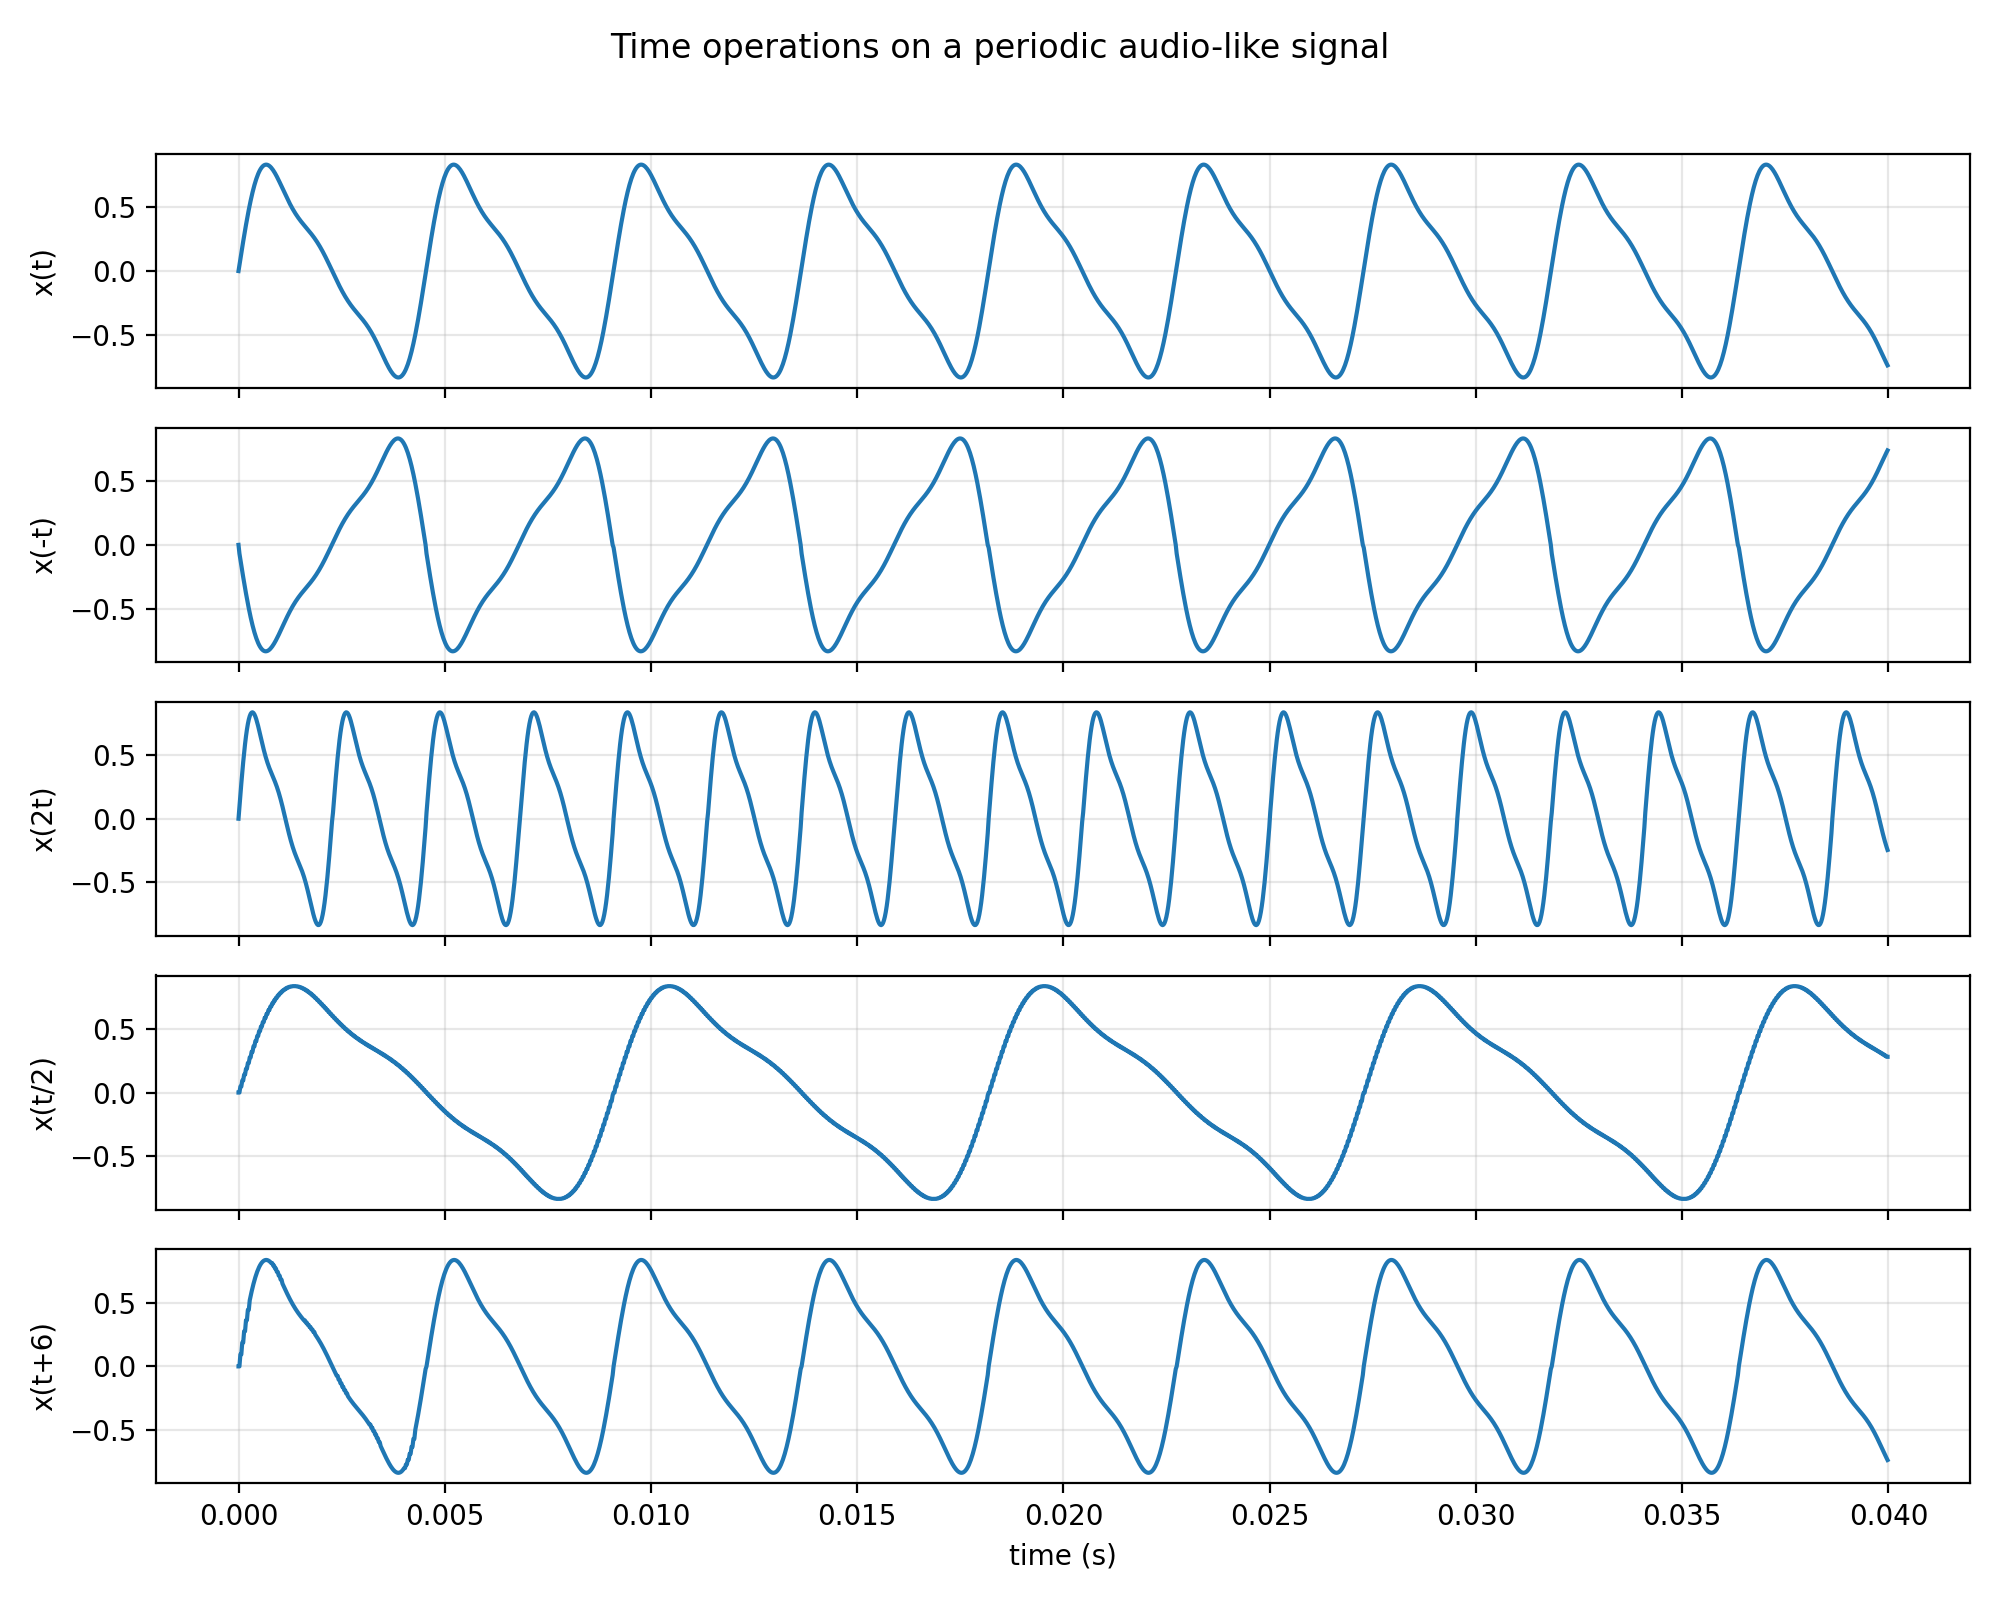
\includegraphics[width=\linewidth]{figs/week2_ops.png}
  \caption{Time operations on a short audio-like signal $x(t)$.}
    \label{fig:week2_ops}
\end{figure}
\begin{figure}[h]
  \centering
  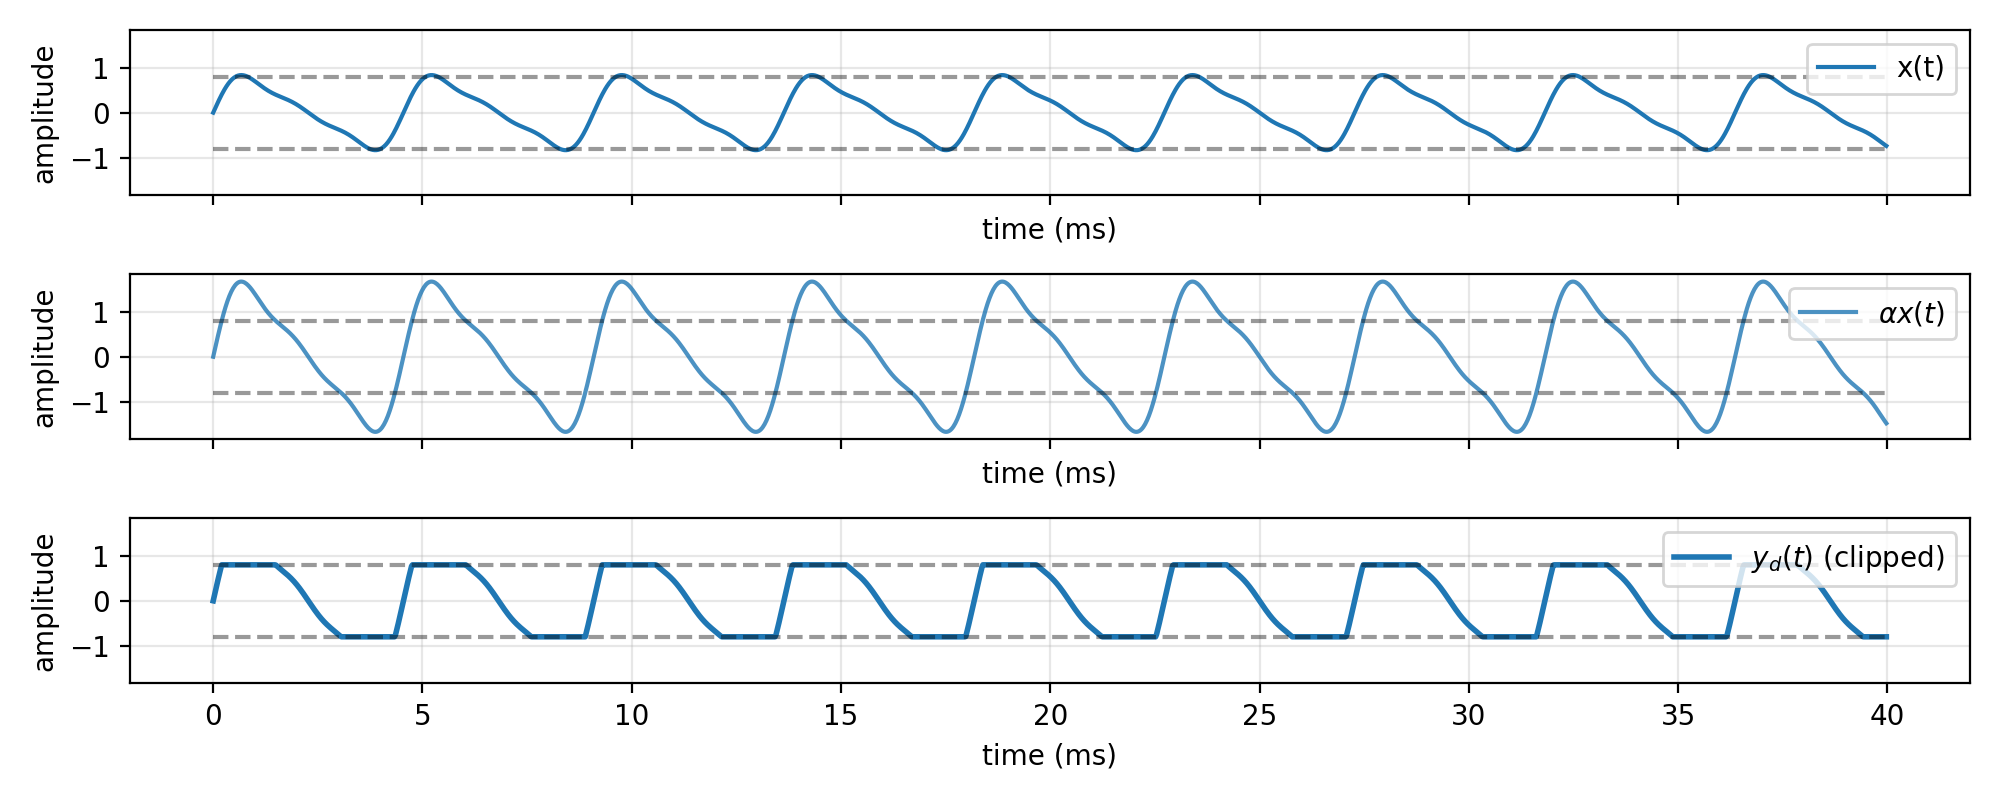
\includegraphics[width=\linewidth]{figs/week2_clip.png}
  \caption{Clipping demo: input $x(t)$, scaled $\alpha x(t)$, and clipped output $y_d(t)$.}
  \label{fig:week2_clip}
\end{figure}


\section{Periodic signals and fundamental period}
A signal $x(t)$ is periodic if $\exists\,T_0>0$ such that $x(t+T_0)=x(t)$ for all $t$. The smallest such $T_0$ is the \emph{fundamental period}. For periodic $x$,
\[
P_\infty(x)=\frac{1}{T_0}\!\int_{t_0}^{t_0+T_0}\!|x(t)|^2 dt
\quad(\text{independent of }t_0),\qquad
E_\infty(x)=\infty\ \text{unless }x\equiv 0.
\]
\textit{A useful trick:} When a signal is defined on a finite interval (e.g., a single cycle), it is often useful to \emph{periodically extend} it by repeating that interval end-to-end. This makes the time-average power well defined and makes symmetries/harmonics easier to see. Memoryless nonlinearities (like clipping) do not change $T_0$ but \emph{do} add harmonics (distortion) while preserving periodicity.

\subsection*{Energy and power for a periodic input}
If $x(t)$ is periodic with fundamental period $T_0$, then $y_d(t)$ is also periodic with the \emph{same} $T_0$ (memoryless mapping preserves period). Hence
\[
E_\infty(y_d)=\int_{-\infty}^{\infty}\!|y_d(t)|^2\,dt=\infty,\qquad
P_\infty(y_d)=\frac{1}{T_0}\int_{t_0}^{t_0+T_0}\!|y_d(t)|^2\,dt\ \text{(finite)}.
\]
For a finite-duration input, $E_\infty$ is finite and $P_\infty=0$ (time average over an unbounded window goes to zero).

\section{Even and odd signals}
A signal $x(t)$ can be decomposed uniquely as
\[
x(t)=x_e(t)+x_o(t),\qquad
x_e(t)=\frac{x(t)+x(-t)}{2},\quad
x_o(t)=\frac{x(t)-x(-t)}{2}.
\]
\textit{Properties.} $x_e$ is even ($x_e(-t)=x_e(t)$), $x_o$ is odd ($x_o(-t)=-x_o(t)$), and $x_e\perp x_o$ in the energy inner product.\\
\textit{Clipping intuition.} The hard–clipper $f(u)=\mathrm{clip}(u,\!-\beta,\beta)$ is an \emph{odd} nonlinearity ($f(-u)=-f(u)$). Thus, if $x$ is even, $y_d$ is generally neither even nor odd; if $x$ is odd, then $y_d$ remains odd.

\section{Complex exponential signals}
\subsection*{Continuous time}
\[
x(t)=A\,e^{j(\omega_0 t+\phi)}=A\cos(\omega_0 t+\phi)+j\,A\sin(\omega_0 t+\phi).
\]
Real and imaginary parts are orthogonal sinusoids. Fundamental period $T_0=\frac{2\pi}{\omega_0}$.

\subsection*{Discrete time}
\[
x[n]=A\,e^{j(\Omega_0 n+\phi)}.
\]
This is periodic iff $\dfrac{\Omega_0}{2\pi}=\dfrac{M}{N}$ with integers $M,N$ coprime. Then the fundamental period is $N_0=N$. Otherwise, it is \emph{aperiodic} on $\mathbb{Z}$.

\subsection*{Geometric (phasor) picture}
The complex exponential traces a circle of radius $A$ in the complex plane at angular speed $\omega_0$ (continuous) or advances by a fixed angle $\Omega_0$ per sample (discrete). The real part is the projection on the horizontal axis; the imaginary part is the vertical projection.

\section*{Next class}
The unit impulse $\delta(t)$ and step $u(t)$; convolution preview.

\end{document}
